\def\tutdate{25.10.2018}

\documentclass{beamer}
\usepackage{../templates/beamerthemekit}
%\usepackage{enumitem}

\usepackage[utf8]{inputenc}
\usepackage[T1]{fontenc}
\usepackage[ngerman]{babel}
\usepackage{listings}
\usepackage{hyperref}
\usepackage{graphicx}

\usepackage{amsmath}
\usepackage{amsthm}
\usepackage{amssymb}
\usepackage{polynom}

%\usepackage{ifthen}
%\usepackage{adjustbox} % for \adjincludegraphics

%\usepackage{tikz}
\usepackage{listings}

%\usepackage[]{algorithm2e}

%\usepackage{colortbl}
\usepackage{verbatim}
%\usepackage{alltt}
%\usepackage{changes}

%\usepackage{pdfpages}
%\usepackage{tabularx}

%\usepackage{euler}


\newcommand{\markBlue}[1]{\textcolor{kit-blue100}{#1}}
\newcommand{\markGreen}[1]{\textcolor{kit-green100}{#1}}
\newcommand{\vertspace}{\vspace{.2cm}}

%\newcommand{\#}{\markBlue{#1}}

%\newcommand{\pitem}{\pause\item}
\newcommand{\p}{\pause}

% -- MATH MACROS
\newcommand{\thistheoremname}{}
\newcommand{\G}{\mathbb{Z}}
\newcommand{\B}{\mathbb{B}}
\newcommand{\R}{\mathbb{R}}
\newcommand{\N}{\mathbb{N}}
\newcommand{\Q}{\mathbb{Q}}
\newcommand{\C}{\mathbb{C}}
\newcommand{\Z}{\mathbb{Z}}
\newcommand{\F}{\mathbb{F}}
\newcommand{\mi}{\mathrm{i}}
\renewcommand{\epsilon}{\varepsilon}
\newcommand{\okalk}{\mathscr{O}}


\newenvironment<>{taskblock}[1]{%
	\setbeamercolor{block title}{fg=kit-orange15,bg=kit-orange100}
	\setbeamercolor{block body}{fg=black,bg=kit-orange30}%
	\begin{block}#2{#1}}{\end{block}}

\setbeamertemplate{enumerate items}[default]

% Aussagenlogik Symbole
\newcommand{\W}{w}
\renewcommand{\F}{f}

% Kodierung
\newcommand{\frepr}{\textbf{repr}}
\newcommand{\fRepr}{\textbf{Repr}}
\newcommand{\fZkpl}{\textbf{Zkpl}}
\newcommand{\fbin}{\textbf{bin}}
\newcommand{\fdiv}{\textbf{ div }}
\newcommand{\fmod}{\textbf{ mod }}

% Speicherabbild
\newenvironment{memory}{\begin{tabular}{r | l}Adresse&Wert\\\hline\hline}{\end{tabular}}
\newcommand{\memrow}[2]{#1 & #2 \\\hline}

% Praedikatenlogik
\newcommand{\objequiv}{\stackrel{\cdot}{=}}
\newcommand{\pval}{val_{D,I,\beta}}

% Neue Befehle
\newcommand{\ip}{\pause} % inline pause, für mitten im satz
\newcommand{\pitem}{\pause\item} % für aufzählungen
\newcommand{\bp}{\pause} % block pause, für zwischen blöcken
\title[Grundbegriffe der Informatik]{ICPC\\Gruppe 2}
\date{\tutdate}
\subtitle{\tutTitle}
\author{Elias Schaut, Dennis Kobert, Niklas Kniep, Lam Vo, Ilia Bozhinov}

\institute{}

\titleimage{bg}
%\titleimage{bg-advent}

%
\ifthenelse{\equal{\compiletype}{livebeamer}}
	{
		\def\livebeamermode{1}
	}{}

\ifthenelse{\equal{\compiletype}{print}}
	{
		\def\printmode{1}
	}{}

\setbeamercovered{invisible}

%\usepackage[citestyle=authoryear,bibstyle=numeric,hyperref,backend=biber]{biblatex}
%\addbibresource{templates/example.bib}
%\bibhang1em

	
\def\tutTitle{Organisatorisches/Grundlagen}
\begin{document}

\selectlanguage{ngerman}

%title page
\begin{frame}
	\titlepage
\end{frame}

\section{Organisatorisches}

\begin{frame}{Termine}
	\begin{itemize}
		 
		\item Vorlesung und Übung
			\begin{itemize}
				\item Mittwoch 9:45 - 11:15 Vorlesung
				\item Freitag 9:45 - 11:15 Vorlesung/Übung
			\end{itemize}
		
		 
		\item Tutorium
			\begin{itemize}
				\item Donnerstags, 15:45 - 17:15
				\item 50.34 Informatikbau, -107
			\end{itemize}
		
		 
		\item Übungsblätter
		\begin{itemize}
			\item Jede Woche
			\item Ausgabe Mittwochs, Abgabe Freitags bis 12:30 eine Woche drauf 
		\end{itemize}
		 
		\item Klausur
		\begin{itemize}
			\item Termin am 19.03.2018 11:00-13:00
		\end{itemize}
	\end{itemize}
\end{frame}

\begin{frame}{Übungsschein}
	\begin{itemize}
		 
		\item min. 50\% aller Punkte auf Übungsblättern richtig 
		\item Rückgabe im Tutorium 
		\item Bestehen ist \emph{keine} Voraussetzung für die Klausur, \emph{aber} fürs Modul! 
		\item Gemeinsames Abgeben, Abschreiben verboten 
		\item Übungsblätter und später auch Musterlösungen im ILIAS
	\end{itemize}
\end{frame}

\begin{frame}{Tutorium}
	\begin{itemize}
		\item Alle Tutorienfolien im Ilias (nach dem Tutorium)
	\end{itemize}
	 
	
	\begin{itemize}
		\item Bei Fragen:uxkln@student.kit.edu 
		\item Oder einfach hier
		\item Keine Anwesenheitspflicht 
		\item Möglichkeit andere Tutorien zu besuchen
	\end{itemize}
\end{frame}


\section{Signale und Nachrichten}

\begin{frame}{Signale und Nachrichten}
	\begin{itemize}
		 \item Objekt: \markBlue{101}
		\begin{itemize}
			 \item Eins null eins oder 101 als Zahl oder 5 in binär oder zwei merkwürdige Striche mit einem Kreis dazwischen?
			 \item Vom Kontext abhängig.
			 \item Zunächst einfach ein konkretes Objekt.
		\end{itemize}
	\end{itemize}
\end{frame}

\begin{frame}{Signale und Nachrichten}	
	\begin{itemize}
		 \item Signal
		\begin{itemize}
			 \item Physikalische Veränderung
			 \item Lässt sich verschieden interpretieren.
			 \item Beispiele:
			\begin{itemize}
				 \item Notfallalarm in Serverraum\\
				
\includegraphics[width=.1\linewidth]{../images/alarm.jpg}\\
				 \item Für Besucher nur schönes Leuchten
				 \item Für Security die Information, zu kommen
				 \item Für Techniker die Information, Ausrüstung zu holen
			\end{itemize}
		\end{itemize}
		
		 \item Nachricht  : Objekt wie oben, das von Signal unabhängig ist
		\begin{itemize}
			 \item Roter Notfallalarm ist ein anderes Signal als ein blauer Notfallalarm, aber vielleicht dieselbe Nachricht.
		\end{itemize}
	\end{itemize}
\end{frame}

\begin{frame}{Signale und Nachrichten}
	\begin{itemize}
		 \item Der interessante Teil: Informationen
		 \item Bedeutung einer Nachricht
		 \item Der vorher fehlende Kontext.
		 \item Im obigen Beispiel:
		\begin{itemize}
			 \item Rote Alarmleuchte ist ein Signal (blaue Signalleuchte in Raum nebendran vielleicht auch)
			 \item ``Alarm'': Nachricht
			 \item Information: Security soll herkommen, Techniker sollen das Werkzeug bereit halten, Besucher sollten Platz machen.
		\end{itemize}
	\end{itemize}
\end{frame}

\section{Mengen}


\begin{frame}{Mengen}
	\begin{itemize}
		 \item Erster wirklich wichtiger Teil.
	\end{itemize}
\end{frame}

\begin{frame}{Mengen}
	\begin{block}{Definition: Mengen}
		 
		``Unter einer Menge verstehen wir jede
		Zusammenfassung von bestimmten
		wohlunterschiedenen Objekten unserer
		Anschauung oder unseres Denkens (welche die
		Elemente dieser Menge genannt werden) zu einem
		Ganzen.''
	\end{block}
	
	\begin{itemize}
		\item Beispiel: $\{a, b, c, d\}$ $ =: A,$ $\{a, c, 4\} =: B, \{10, 11\} =: C$
		\item Das Objekt $c$ ist in $A$ enthalten  : $c \in A$  , $c \in B$  , $c \notin C$
		\item Reihenfolge gleich  : $\{a, b\} = \{b, a\}$
		\item Elemente doppelt?   $\{a, a, b, a\} = \{a, b\}$
	\end{itemize}
\end{frame}

\begin{frame}{Mehr über Mengen}
	\begin{itemize}
		\item Kardinalität   oder Größe  : Die Anzahl der Elemente der Menge
		\begin{itemize}
			\item $A := \{a, b, c\}$  . $|A| = 3$
			\item $B := \{c, d\}$  . $|B| = 2$
			\item Was ist $|\{1, 2, 3, 2\}|$?   $3$!
			\item Was ist $|\emptyset|?$   $0$
		\end{itemize}
	\end{itemize}
	
	 
	
	\begin{block}{Leere Menge}
		Die Menge, die nichts enthält, nennen wir die leere Menge  , und schreiben sie als $\{\}$ oder $\emptyset$.
	\end{block}
	
	 
	
	Was ist $|\{\emptyset\}|$?   1!   $\{\emptyset\}$ enthält eine leere Menge, die selbst ein Element ist.
\end{frame}


\begin{frame}{Mehr über Mengen}
	  Seien $A := \{a, b, c\}, B:= \{b, c\}, C:= \{c, b\}, D := \{b, c, d\}$.
	
	\begin{itemize}
		\item Teilmenge  : $A \subseteq B$  , also $A$ ist Teilmenge von $B$   genau dann, wenn alle Elemente aus $A$ auch in $B$ sind.
		\item Echte Teilmenge  : $A \subset B$   genau dann, wenn $A \subseteq B$   \emph{und} $A \neq B$.
		\begin{itemize}
			\item Beispiele:   $B \subseteq A$  , sogar $B \subset A$.\\   $C \subseteq B$   und $B \subseteq C$  , aber $C \not\subset B$ und $B \not\subset C$.
		\end{itemize}
		\item Schnittmenge  : $A \cap B$   $ = \{b, c\}$.  \\ $A \cap B$ enthält \emph{genau} die Elemente, die in $A$ \emph{und} in $B$ sind.%TODO erkläre "genau", siehe LA. Wieso übrigens kein := ?
		\item Vereinigungsmenge  : $A \cup D$   $ = \{a, b, c, d\}$.  \\ $A \cup B$ enthält \emph{genau} die Elemente, die in $A$ \emph{oder} in $B$ sind.
		\item Mengendifferenz:   $A \setminus B$   $ = \{a\}$  , also alle Elemente in $A$, die nicht in $B$ sind.  
	\end{itemize}
\end{frame}

\begin{frame}{Rechenregeln für Mengen}
	\begin{itemize}
			\item $A \setminus B = \emptyset$  bedeutet das gleiche wie $A \subseteq B$
			\item $ \{1, 2, 3\} \cup \{2, 3, 4\} = \{1, 2, 3, 4\}$
			\item $ M \cup \emptyset = M $
			\item $ M \cap \emptyset = \emptyset $
			\item $ A \cup (B \cup C) = (A \cup B) \cup C $ (analog für Durchschnitt)
			\item $ A \cup (B \cap C) = (A \cup B) \cap (A \cup C) $ (analog Vertauschen von $\cup$ und $\cap$)
			\item $|A \cup B| = |A| + |B| - |A \cap B|$
	\end{itemize}
\end{frame}

\begin{frame}{Potenzmenge}
	 
	
	\begin{block}{Potenzmenge}
		Die Potenzmenge   $2^M$   einer Menge $M$   enthält genau alle Mengen, die Teilmenge von $M$ sind.	
	\end{block}
	
	 
	
	Was bedeutet das allgemein?
	
	\begin{itemize}
		\item $M \in 2^M$
		\item $\emptyset \in 2^M$
		\item Konkretes Beispiel:   Was ist $2^M$ mit $M = \{0, 1\}$?
		\begin{itemize}
			\item Natürlich $\emptyset \in 2^M$ und $\{0, 1\} \in 2^M$.
			\item $\{0\} \in 2^M$   und $\{1\} \in 2^M$.
			\item Weitere?   Nein, diese vier Mengen sind alle möglichen Teilmengen.
			\item $\Rightarrow$ $2^M = \{\{\}, \{0\}, \{1\}, \{0, 1\}\}$.
		\end{itemize}
	\end{itemize}
\end{frame}

\begin{frame}{Potenzmenge}
	$M = \{0, 1\}$  , $2^M = \{\{\}, \{0\}, \{1\}, \{0, 1\}\}$. 
	
	Was ist $2^{2^M}$?
	
	\begin{itemize}
		\item Also $2^{\{\{\}, \{0\}, \{1\}, \{0, 1\}\}}$.
		\item Natürlich $\emptyset \in 2^M$ und $2^M = \{\{\}, \{0\}, \{1\}, \{0, 1\}\} \in 2^{2^M}$.
	\end{itemize}
	
	 
	
	$2^{2^M}  
	= 
	\{  $\\$ \quad
	\{\},$\\$ \quad
	\{\{\}\}, 
	\{\{0\}\}, 
	\{\{1\}\},
	\{\{0, 1\}\}, $\\$ \quad
	\{\{\}, \{0\}\}, 
	\{\{\}, \{1\}\}, 
	\{\{\}, \{0, 1\}\}, 
	\{\{0\}, \{1\}\}, $\\$\qquad
	\{\{0\}, \{0, 1\}\}, 
	\{\{1\}, \{0, 1\}, $\\$ \quad
	\{\{\}, \{0\}, \{1\}\}, 
	\{\{\}, \{0\}, \{0, 1\}\}, 
	\{\{\}, \{1\}, \{0, 1\}\}, 
	\{\{0\}, \{1\}, \{0, 1\}\}, $\\$ \quad
	\{\{\}, \{0\}, \{1\}, \{0, 1\}\} $\\$
	\}
	$
\end{frame}

\section{Alphabete}
\begin{frame}{Alphabete}
	
	 
	
	\begin{block}{Alphabet}
		Ein Alphabet ist eine \emph{endliche}, \emph{nichtleere} Menge von Zeichen.
	\end{block}
	
	 
	
	Was davon sind Alphabete?   $\{d, 34, \pi, \%\}$  , $\{a, b, c, \dots, y, z\}$  , $\emptyset$  , $\N$.
	
	\begin{itemize}
		\item $\{d, 34, \pi, \%\}$ und $\{a, b, c, \dots, y, z\}$ sind Alphabete.
		\item $\emptyset$ ist leer und damit kein Alphabet.
		\item $\N = \{1, 2, 3, \dots\}$ enthält alle natürlichen Zahlen und ist damit nicht endlich, also kein Alphabet.
		\item $\{0, 1\}$ ist das Alphabet, das alle Binärzahlen enthält.
		\item $\{\cdot, +, -, /\} =: R$ ist ein Alphabet von Rechenzeichen.  $R \cup \{0, 1, \dots, 9\}$ ist ein Alphabet, das ein Taschenrechner als Eingabealphabet benutzen könnte.
	\end{itemize}
\end{frame}

\section{Relationen und Abbildungen}
\begin{frame}{Paare und Tupel}
	 
	\begin{block}{Paar}
		Ein Paar ist eine geordnete Menge der Kardinalität 2.
	\end{block}
	 
	Schreibweise mit runden Klammern ().
	\begin{itemize}
		\item Beispiel: $(a, 4)$  $\neq (4, a)$
		\item Beispiel für eine Menge aus Tupeln: $\{(Star Wars, Sci-Fi),$ $(Harry Potter, Fantasy),$ $(Fight Club, Thriller)\}$
	\end{itemize}
\end{frame}

\begin{frame}{Tupel}
	 
	\begin{block}{Tupel}
		Ein Tupel ist eine geordnete Menge.   Konkret ist ein $n$-Tupel ein Tupel der Kardinalität $n$.
	\end{block}
	 
	Also wie ein Paar, nur mit beliebiger Kardinalität.   Ein Paar ist spezifisch ein 2-Tupel. 
	
	Beispiel: $(4tb, 512gb, 128gb, 4mb)$   $\neq (512gb, 4mb, 4tb, 128gb)$.
\end{frame}

\begin{frame}{Kartesisches Produkt}
	Zwei Mengen: $A := \{a, b, c\}$   und $B := \{1, 2, 3\}$.  
	
	Wir wollen alle Tupel   mit erstem Element aus $A$   und zweiten Element aus $B$. 
	
	$\{
	\quad (a, 1), (a, 2), (a, 3), 
	\qquad (b, 1), (b, 2), (b, 3), 
	\qquad (c, 1), (c, 2), (c, 3)\quad
	\}$   $ = A \times B$
	
	 
	
	\begin{block}{Kartesisches Produkt von zwei Mengen}
		Zu zwei Mengen $A$ und $B$ ist das kartesische Produkt definiert als Menge aller Paare $(a, b)$ mit $a \in A$ und $b \in B$.
	\end{block}
\end{frame}

\begin{frame}{Kartesisches Produkt}
	\begin{block}{Kartesisches Produkt von zwei Mengen}
	Zu zwei Mengen $A$ und $B$ ist das kartesische Produkt $A \times B$ definiert als Menge aller Paare $(a, b)$ mit $a \in A$ und $b \in B$.
	\end{block}
	
	\begin{block}{Kartesisches Produkt von n Mengen}
		Zu $n$ Mengen $M_1$, $M_2$, \dots, $M_n$   ist das Kreuzprodukt $M_1 \times M_2 \times \cdots \times M_n$   definiert als Menge aller $n$-Tupel $(e_1, e_2, \dots, e_n)$   mit $e_1 \in M_1$, $e_2 \in M_2$, \dots, $e_n \in M_n$.
	\end{block} 
	
	\begin{block}{Mengenpotenz}
		$\underbrace{A \times A \times \cdots \times A}_{n \times mal} = A^n$.
	\end{block}
\end{frame}

\begin{frame}{Kartesisches Produkt: Beispiele}
	\begin{block}{Kartesisches Produkt von zwei Mengen}
		Zu zwei Mengen $A$ und $B$ ist das kartesische Produkt $A \times B$ definiert als Menge aller Paare $(a, b)$ mit $a \in A$ und $b \in B$.
	\end{block}
	 
	
	$A := \{a, b\}, B := \{1, 2\}$.   $A \times B$   $ = \{(a, 1), (a, 2), (b, 1), (b, 2)\}$.
\end{frame}

\begin{frame}{Kartesisches Produkt: Beispiele}
	
	\begin{block}{Kartesisches Produkt von n Mengen}
		Zu $n$ Mengen $M_1$, $M_2$, \dots, $M_n$   ist das kartesische Produkt $M_1 \times M_2 \times \cdots \times M_n$   definiert als Menge aller $n$-Tupel $(e_1, e_2, \dots, e_n)$   mit $e_1 \in M_1$, $e_2 \in M_2$, \dots, $e_n \in M_n$.
	\end{block} 
	
	$A := \{a, b\}, B := \{1, 2\}, C:= \{\omega\}$. $A \times B \times C$   $ = \{(a, 1, \omega), (a, 2, \omega), (b, 1, \omega), (b, 2, \omega) \}$.
	
\end{frame}

\begin{frame}{Kartesisches Produkt: Beispiele}
	
	\begin{block}{Mengenpotenz}
		$\underbrace{A \times A \times \cdots \times A}_{n mal} = A^n$.
	\end{block} 
	
	\begin{itemize}
		\item $A := \{a, b\}$.   $A^2$   $ = \{(a, b), (b, a), (a, a), (b, b)\}$   $A^3 = \{(a, a, a), (a, a, b), (a, b, b), \dots\}$.
		\item $A$ beliebige Menge.   $A^0$?   $ = \emptyset$ 
		\item Achtung! $2^M \neq M^2$.   Potenzmengen nicht mit Mengenpotenz verwechseln!
	\end{itemize}
	
\end{frame}

\begin{frame}{Relation}
	 
	
	\begin{block}{Binäre Relation}
		Eine binäre Relation auf zwei Mengen $A$ und $B$ ist eine Menge $R \subseteq A \times B$.
	\end{block} 
	
	\begin{itemize}
		\item Für die Mengen $M_{Filme} = \{Star Wars, Harry Potter, Fight Club\}$, $M_{Genre} = \{Sci-Fi, Fantasy, Thriller\}$ sind folgendes mögliche Relationen:
		\begin{itemize}
			\item $\{(Star Wars, Sci-Fi),$ $(Harry Potter, Fantasy),$ $(Fight Club, Thriller)\}$
			\item $\{(Star Wars, Sci-Fi), (Fight Club, Thriller)$
			\item $\emptyset$
		\end{itemize}
		\item ``Kleinergleichrelation'' auf $M = \{1, 2, 3\}$  : $R_\leq = \{(1, 1), (1, 2), (1, 3), (2, 2), (2, 3), (3, 3)\}$   $\subseteq M \times M$
	\end{itemize}
\end{frame}


\begin{frame}{Relation}
	\begin{block}{Binäre Relation}
		Eine binäre Relation auf zwei Mengen $A$ und $B$ ist eine Menge $R \subseteq A \times B$.
	\end{block} 
	
	\begin{block}{Ternäre Relation}
		Eine ternäre Relation auf drei Mengen $A$, $B$ und $C$ ist eine Menge $R \subseteq A \times B \times C$.
	\end{block} 
	
	\begin{block}{n-äre Relation}
		Eine $n$-äre Relation auf $n$ Mengen $M_1$, $M_2$ ... $M_n$ ist eine Menge $R \subseteq M_1 \times M_2 \times \cdots \times M_n$.
	\end{block}
\end{frame}

\begin{frame}{Linkstotalität}
	\begin{block}{Linkstotale Relation}
		Eine Relation $R \subseteq A \times B$ heißt linkstotal  , wenn für jedes $a \in A$ ein $b \in B$ existiert mit $(a,b) \in R$.
	\end{block} 
	
	Die linke Seite der Relation ist also ``total'' aufgefüllt. 
	
	\begin{center}
		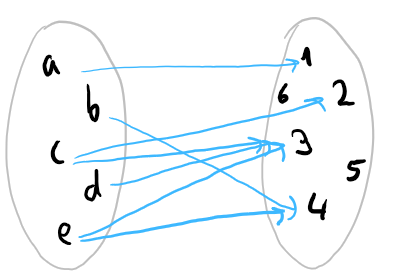
\includegraphics[width=.5\linewidth]{../images/mengen_linkstotal.png}
	\end{center}
\end{frame}

\begin{frame}{Rechtstotalität}
	\begin{block}{Rechtstotale Relation}
		Eine Relation $R \subseteq A \times B$ heißt rechtstotal, wenn für jedes $b \in B$ ein $a \in A$ existiert mit $(a,b) \in R$.
	\end{block} 
	
	Die rechte Seite der Relation ist also ``total'' aufgefüllt. 
	
	\markGreen{Wenn die Relation zusätzlich eine Abbildung ist, heißt diese dann} \markBlue{surjektiv}. 
	
	\begin{center}
		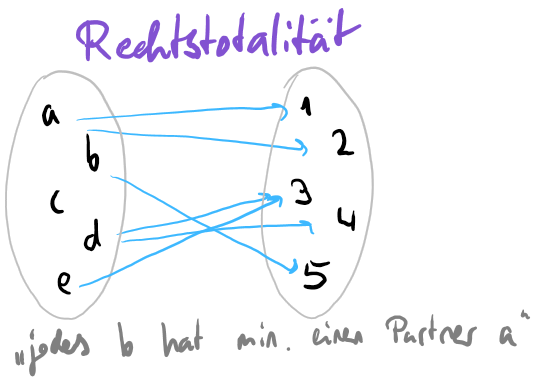
\includegraphics[width=.5\linewidth]{../images/mengen_rechtstotal.png}
	\end{center}
\end{frame}

\begin{frame}{Linkseindeutigkeit}
	\begin{block}{Linkseindeutige Relation}
		Eine Relation $R \subseteq A \times B$ heißt linkseindeutig, wenn für zwei beliebige Elemente $(a, \alpha) \in R, (b, \beta) \in R$ aus der Relation $R$ gilt: wenn $a \neq b$, dann gilt auch $\alpha \neq \beta$. 
	\end{block} 
	
	Also: Keine zwei Elemente der linken Seite der Relation haben dasselbe rechte Element. 
	
	Angenommen, $a \neq b$ und $\alpha = \beta$.   $\Rightarrow$ offenbar nicht linkseindeutig.
	
	\markGreen{Wenn die Relation zusätzlich eine Abbildung ist, heißt diese dann} \markBlue{injektiv}.
	
	\begin{center}
		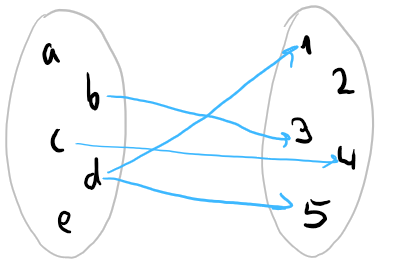
\includegraphics[width=.4\linewidth]{../images/mengen_linkseindeutig.png}
	\end{center}
\end{frame}

\begin{frame}{Rechtseindeutig}
	\begin{block}{Rechtseindeutige Relation}
		Eine Relation $R \subseteq A \times B$ heißt rechtseindeutig , wenn für zwei beliebige Elemente $(a, \alpha) \in R, (b, \beta) \in R$ aus der Relation $R$ gilt: wenn $\alpha \neq \beta$, dann gilt auch $a \neq b$. 
	\end{block}
	
	Also: Keine zwei Elemente der rechten Seite der Relation haben dasselbe linke Element.
	
	\begin{center}
		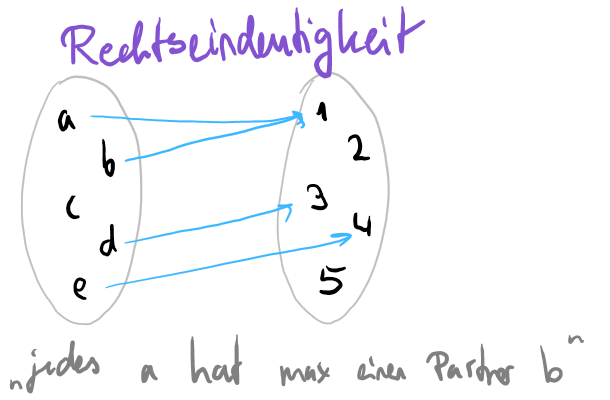
\includegraphics[width=.5\linewidth]{../images/mengen_rechtseindeutig.png}
	\end{center}
\end{frame}

\ifdefined\printmode
\begin{frame}{Eigenschaften von Relationen}
	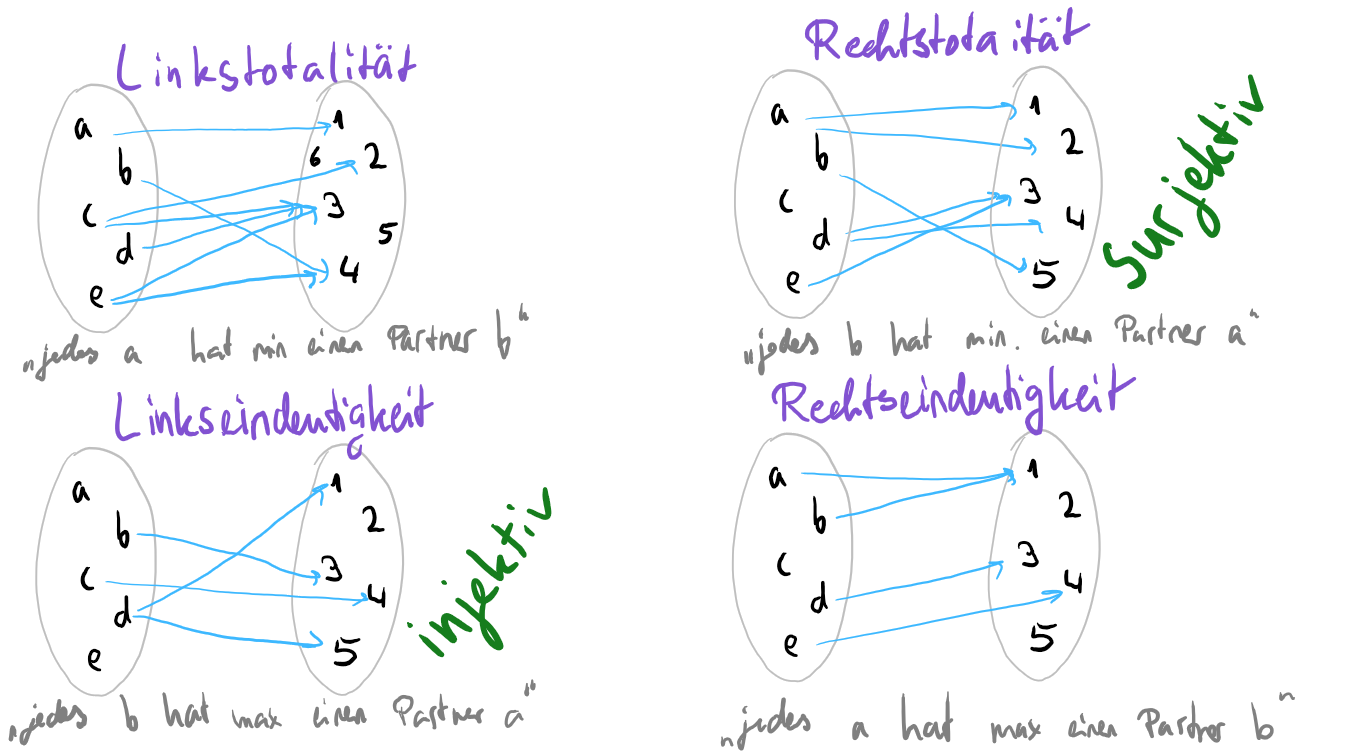
\includegraphics[width=\linewidth]{../images/mengen_alle.png}
\end{frame}
\fi

\begin{frame}{Abbildung}
	\begin{block}{Abbildung}
		Eine Relation $R$ heißt eine Abbildung, wenn sie linkstotal \emph{und} rechtseindeutig sind.
	\end{block}
	
	\begin{itemize}
		\item Injektive Funktion: \markGreen{linkstotal}, \markGreen{rechtseindeutig}, \markBlue{linkseindeutig}
		\item Surjektive Funktion: \markGreen{linkstotal}, \markGreen{rechtseindeutig}, \markBlue{rechtstotal}
	\end{itemize}
	
	
	\begin{block}{Bijektivität}
		Eine Relation heißt bijektiv, wenn sie injektiv und surjektiv ist.
	\end{block}
	
	Damit ist sie \markGreen{linkstotal} und \markGreen{rechtseindeutig} (weil es eine Abbildung ist) und \markBlue{linkseindeutig} (injektiv) und \markBlue{rechtstotal} (surjektiv).
	
	  Tolle Eigenschaft:   Für jedes Element $(a, b) \in R$ der bijektiven Relation $R$ ist \emph{jedem} $a$ \emph{genau ein} $b$ zugeordnet. 
	
\end{frame}

\begin{frame}{Abbildungen Schreibweise}
	Seien $A = B = \R$, $f \subseteq A \times B$.   Wir suchen Relation, die für jedes $a \in A$ ein Element $(a, b) \in f$ enthält mit $b = a^2$. 
	
	$f = \{(0, 0), (0.1, 0.01), (2, 4), \dots\}$ 
	
	  Unendlich viele Elemente, und unmöglich alle zu nennen.
	
	 (Mathematischere) Schreibweise für Abbildungen: 
	
	$f : A \rightarrow B, a \mapsto a^2$  , also Quadratfunktion.
	
	  Ist diese Funktion injektiv oder surjektiv?   
	
	\begin{itemize}
		\item Nicht injektiv, da z.B. $f(1) = f(-1)$  , also $(1, 1) \in f$ und $(-1, 1) \in f$. 
		\item Nicht surjektiv, da z.B. $-1$ nie als Funktionswert angenommen wird  , daher $(a, -1) \not\in f$ für beliebige $a \in A$.
	
	\end{itemize}
	
\end{frame}


\begin{frame}
	
\includegraphics[width=\linewidth]{../images/thatsall.png}
\end{frame}


\end{document}